\documentclass[a4paper,oneside,12pt]{report}

\usepackage[utf8]{inputenc}
\usepackage[T1]{fontenc}
\usepackage[french]{babel}
\usepackage{hyperref}
\usepackage[official]{eurosym}
\usepackage{stageutc}

\newcommand{\cf}[1]{cf. #1}
\newcommand{\etranger}[1]{\textit{#1}}

\newcommand{\refsection}[1]{section~\ref{section:#1}}
\newcommand{\cfsection}[1]{\cf{\refsection{#1}}}

\newcommand{\reffigure}[1]{figure~\ref{figure:#1}}
\newcommand{\cffigure}[1]{\cf{\reffigure{#1}}}


\newcommand{\acentreon}{Centreon}
\newcommand{\alinotp}{LinOTP}
\newcommand{\aintranet}{Intranet}
\newcommand{\atypo}{Typo3}
\newcommand{\aad}{Microsoft Active Directory}
\newcommand{\aradius}{RADIUS}
\newcommand{\afreerad}{FreeRADIUS}

\newcommand{\asmile}{Smile}
\newcommand{\abusys}{BU Système}
\newcommand{\abugan}{BU Ganesh}
\newcommand{\alse}{LSE}

\newcommand{\ame}{Jérémy Subtil}
\newcommand{\apakou}{Patrick Kouassi}
\newcommand{\asuiveur}{Dritan Nace}
\newcommand{\amabes}{Maxime Besson}
\newcommand{\agulet}{Guilhem Lettron}
\newcommand{\asegir}{Sébastien Giraud}
\newcommand{\amimiette}{Philippe Mimiette}
\newcommand{\ahbt}{Hervé Brassart}
\newcommand{\arolel}{Romain Leleu}



\title{TN10 -- Rapport de stage}
\subtitle{Ingénieur système et développement en environnement open source}
\author{\ame}
\date{Semestre~P11}

\makeatletter
\hypersetup{
	pdftitle={\@title},
	pdfauthor={\@author},
	pdfsubject={\@subtitle}
}
\makeatother

\graphicspath{{figs/}}


\begin{document}

\maketitle

\section*{Remerciements}

Je souhaite remercier \apakou, directeur de la \abusys, qui m'a accueilli dans son équipe chez \asmile{} et qui a suivi mon évolution au cours de ces six mois de stage.

Je remercie également mon maître de stage \agulet, ingénieur système, pour m'avoir guidé tout au
long du stage, m'avoir appris un tas de choses et m'avoir payé quelques verres.

Je voudrais aussi exprimer ma gratitude envers \amabes, expert technique système, qui m'a toujours accordé du temps pour répondre à mes questions.

Je remercie également \asuiveur, mon tuteur de stage de l'UTC, pour son soutien.

Enfin, je souhaiterais exprimer mes remerciements envers tous mes collègues titulaires et bizus\footnote{C'est ainsi que l'on surnomme les stagiaires dans la \abusys.} qui m'ont tous toujours bien accueilli parmi eux et avec qui j'ai passé d'excellents moments.


\newpage

\tableofcontents
\listoffigures
\newpage

\section*{Résumé technique}

TODO


\newpage

% fancyhdr
\pagestyle{fancy}
\lhead{\begin{small}\nouppercase{\leftmark}\end{small}}
\rhead{\begin{small}\nouppercase{\rightmark}\end{small}}

\chapter{Présentation de l'entreprise}

\section{Le groupe \asmile}

\paragraph{}
\asmile{} est une Société de Services en Ingénierie Informatique (SSII) française, dont l'activité principale repose sur le développement web et l'intégration de solutions open source\footnote{La désignation open source s'applique aux logiciels dont la licence respecte des critères précisément établis par l'Open Source Initiative, c'est-à-dire la possibilité de libre redistribution, d'accès au code source et aux travaux dérivés.~\cite{opensource}}.
\asmile{} est d'ailleurs aujourd'hui considérée comme le leader français dans le domaine.

\paragraph{}
La société a été créée en 1991 par quatre fondateurs : Jérôme Prompsy, Patrice Bertrand, Alain Arditi et Cyrille Chignardet.
\asmile{} innove alors dans le domaine des logiciels décisionnels en s'appuyant sur les méthodes de développement RAD (\textit{Rapid Application Development}).
En 1995, l'entreprise prend une nouvelle orientation du fait de la démocratisation d'Internet et des applications web.
Pionnière sur le secteur, \asmile{} se fait notamment connaître par la conception du premier site bancaire sur le web pour le Crédit Lyonnais.

\paragraph{}
En 2001, \asmile{} fait un nouveau choix stratégique en se positionnant sur les technologies open source.
En effet, en 2004, de plus en plus d'entreprises adoptent ce type de solutions qui deviennent populaires.
En 2011, \asmile{} est présent sur plusieurs gammes de produits web tels que les CMS, les portails, l'e-commerce, le décisionnel, l'ERP et l'infrastructure.
En outre, \asmile{} compte de nouveaux secteurs d'activités plus ou moins liés à l'activité du développement web : une agence média, un pôle d'exploitation, un pôle maintenance et un pôle système.

\paragraph{}
Forte de 20 ans d'expérience, \asmile{} a su se développer dans des grandes villes en métropole telles que Lyon, Bordeaux, Montpellier et Nantes.
Actuellement, le groupe continue son expansion en ouvrant d'autres agences à Aix-en-Provence, Poitiers, Grenoble et Lille.
Par ailleurs, \asmile{} manifeste aussi sa présence en Europe, avec les agences de Barcelone, Genève et Amsterdam.
Aujourd'hui, \asmile{} se développe même en dehors de l'Union Européenne, grâce aux agences de Casablanca au Maroc et de Kiev en Ukraine.

L'ensemble de ces sites sont localisés sur la \reffigure{presentation:carte}.

\begin{figure}
	\centering
	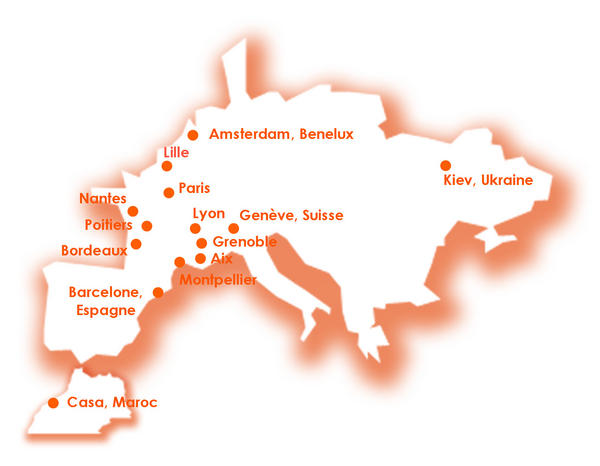
\includegraphics[width=10cm]{presentation/carte-europe-smile}
	\caption{\asmile{} en Europe}
	\label{figure:presentation:carte}
\end{figure}


\paragraph{}
Par ailleurs, l'organisation de \asmile{}, représentée en \reffigure{presentation:organigramme}, est la suivante :

\begin{itemize}
	\item en cyan, la Direction ;
	\item en beige, les BU\footnote{\textit{Business Unit}} de développement web, soit quatre unités sur Paris et quatre réparties en agences en province ;
	\item en bleu, les BU de développement européennes et offshore, qui mènent des projets locaux et des projets expertisés par Paris ;
	\item en vert, les agences métier qui regroupent les offres système, médias ainsi que les formations clients ;
	\item en violet, la BU Consulting qui gère les projets décisionnels et organisationnels.
\end{itemize}

\begin{figure}
	\centering
	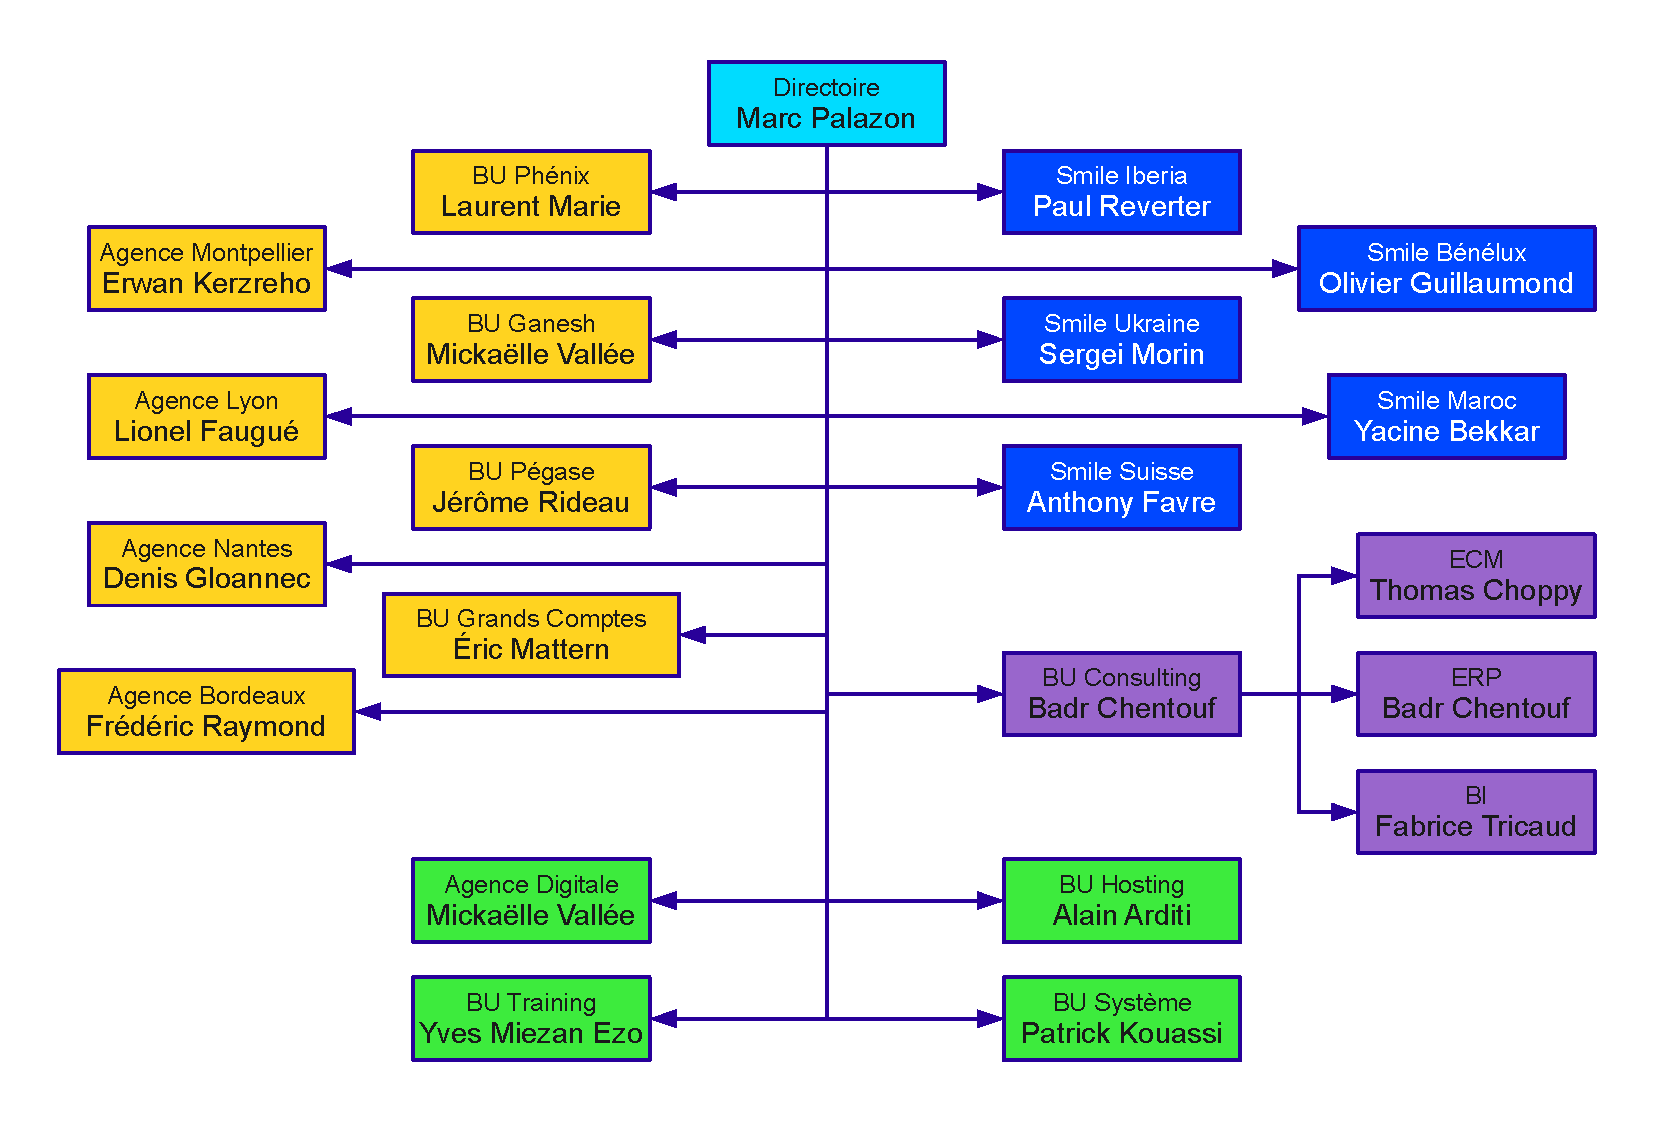
\includegraphics[width=12cm]{presentation/organigramme}
	\caption{Organigramme du groupe \asmile}
	\label{figure:presentation:organigramme}
\end{figure}


\section{Le site parisien}

\paragraph{}
Le site parisien de \asmile{} se situe à Levallois-Perret.
Il est composé de deux bâtiments : l'un est l'ancien bâtiment de Hertford British Hospital, et l'autre un building situé à 300 mètres.
Ces bâtiments accueillent aujourd'hui plusieurs pôles de \asmile{}.

\paragraph{}
Le premier ensemble consiste en le siège social et une partie de l'administration de l'entreprise :

\begin{itemize}
	\item le bureau du Président Directeur Général, Marc Palazon ;
	\item le bureau du Directeur Général, Patrice Bertrand ;
	\item le service des Relations Humaines ;
	\item le service de la communication ;
	\item les services commerciaux ;
	\item le service financier,
	\item le système interne.
\end{itemize}

\paragraph{}
Le second regroupe des équipes métier et développement, qui sont regroupées par clients et technologies maîtrisées :

\begin{description}
	\item[la \abugan{} :] spécialiste PHP, e-commerce avec Magento, expertise CMS avec eZpublish, \atypo{}, Drupal ;
	\item[la BU Pégase :] spécialiste PHP également, e-commerce avec Magento, développement spécifique avec le framework Symfony ;
	\item[la BU Phoenix :] développements spécifiques en Java, CMS avec Jahia ;
	\item[la BU Consulting :] BI, GED, ECM, ERP ;
	\item[la BU Training :] formations ;
	\item[la \abusys{} :] c'est dans cette structure que j'ai pu travailler.
\end{description}


\section{La \abusys{}}

\paragraph{}
La \abusys{} est un pôle de prestation et de conseil dans le domaine des infrastructures système et réseau.
Le rôle de cette équipe est d'accompagner les clients dans le renouvellement et l'optimisation de leurs installations.

\paragraph{}
Pour cela, l'offre système s'articule autour de quatre solutions :

\begin{itemize}
	\item l'aide au management :
	\begin{itemize}
		\item pour les plateformes web ;
		\item pour les infrastructures réseau ;
	\end{itemize}
	\item l'optimisation des infrastructures :
	\begin{itemize}
		\item par mutualisation des ressources grâces à des technologies de virtualisation ;
		\item par des réglages fins des outils suite à des tests de charge ;
	\end{itemize}
	\item la sécurité et gestion des accès utilisateurs :
	\begin{itemize}
		\item authentification ;
		\item VPN ;
		\item firewalls ;
	\end{itemize}
	\item l'étude de solutions haute disponibilité ;
	\item la migration vers des solutions open source :
	\begin{itemize}
		\item re-packaging de distributions Linux ;
		\item solutions de messageries et groupeware ;
		\item VoIP ;
		\item plate-formes d'intégration continue\ldots
	\end{itemize}
\end{itemize}

\paragraph{}
Aussi, la \abusys{} propose une offre interne de support projet pour les autres BU et agences de
\asmile{} :

\begin{itemize}
	\item le déploiement d'environnements de recette pour les projets de développement ;
	\item l'intégration des infrastructures évoluées, comme la haute disponibilité par exemple ;
	\item le soutien aux projets au niveau système.
\end{itemize}

\paragraph{}
Finalement, pour chaque besoin de l'entreprise, la \abusys{} peut proposer une solution open source adaptée.
L'offre système est illustrée en \reffigure{presentation:offre-sys}.

\begin{figure}
	\centering
	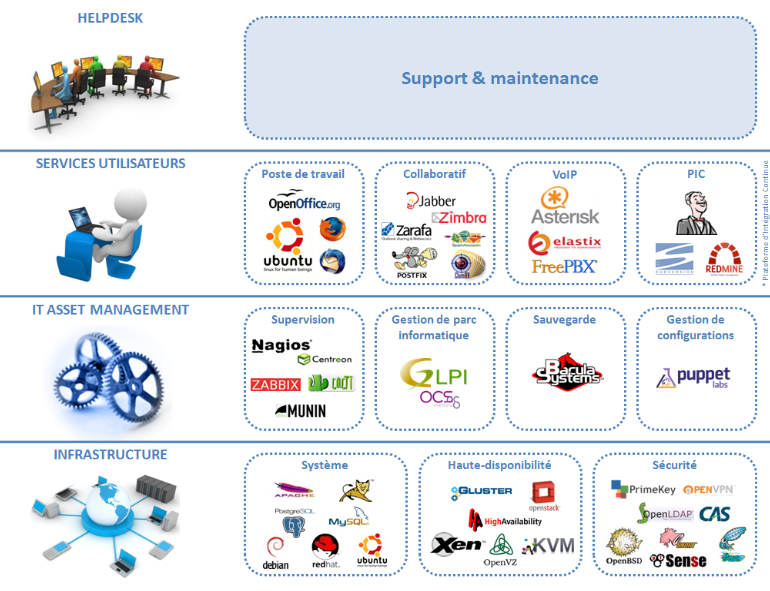
\includegraphics[width=12cm]{presentation/offre-sys}
	\caption{L'offre de la \abusys}
	\label{figure:presentation:offre-sys}
\end{figure}


\chapter{Déroulement du stage}

\section{Ma place au sein de la \abusys}

\paragraph{}
Passionné par l'écosystème de l'open source, c'est naturellement que j'ai choisi de postuler chez \asmile{} pour effectuer mon projet de fin d'études.
Sortant de la filière SRI de l'UTC, j'étais très intéressé de développer mes compétences système et c'est ainsi que j'ai pu intégrer la \abusys{}.

\paragraph{}
Dès mon premier entretien, j'ai défini avec \agulet{}, mon futur tuteur dans l'entreprise, le sujet principal de mon stage : nous avons choisi que je travaille sur les problématiques d'intégration continue.
En effet, à la \abusys{}, c'est une des spécialités de \agulet{}.
Il en est le référent quand il s'agit de fournir une prestation autour de ce domaine pour le compte de clients.
Pour ma part, c'est un sujet qui m'enthousiasme car il fait à la fois intervenir des connaissances en système et en qualité logicielle.
Ainsi, mon travail et ma réflexion sur l'intégration continue et ses outils sont développés dans le \refchap{pic}.

\paragraph{}
Par ailleurs, j'ai eu l'opportunité de travailler de bout en bout sur la mise en place d'une solution d'authentification open source particulière chez un client : \alinotp.
Elle fait intervenir les OTP, ou \etranger{One-Time Passwords}, qui sont en réalité des mots de passe éphémères générés par un matériel tiers.

Cette mission s'est déroulée sur la fin de mon stage, et j'ai alors eu l'opportunité de réaliser un véritable travail d'ingénieur système au même titre que mes collègues titulaires.
Elle est décrite en détail dans le  \refchap{linotp}.

\paragraph{}
En outre, j'ai eu l'occasion de travailler sur une multitude d'autres projets de taille plus ou moins importante :

\begin{itemize}
	\item mettre en place chez un client une solution de supervision \acentreon{} (\cfchap{centreon}) ;
	\item apporter un support d'administration système dit \emph{support projet} aux projets des différentes BU de développement de \asmile{} (\cfchap{support}) ;
	\item apporter un soutien au développement d'un projet client en retard pour \abt{} (développement avec le framework PHP Symfony et le framework JavaScript ExtJS) ;
	\item mettre en place une plateforme web de visioconférence pour \asmile{} avec la solution libre BigBlueButton ;
	\item auditer le code du logiciel libre Linbox-Converter pour le compte de Renault, qui permet de convertir des documents Microsoft Office vers d'autres formats ;
	\item chiffrer des projets système dans le cadre des processus d'avant-vente de \asmile.
\end{itemize}

\paragraph{}
Enfin, j'ai pu commencer certains travaux qui n'ont pas pu aboutir pour diverses raisons.
Ceux-ci sont décrits brièvement en \refsection{avortes}.



\section{Projets avortés}
\label{section:avortes}

TODO



\section{Planning effectif}

\paragraph{Février}
\begin{itemize}
	\item Support projet
	\item Mise en place d'un serveur de base de données Oracle
	\item Auto-formation sur la réplication de bases de données MySQL
	\item Auto-formation sur les outils Hudson/Jenkins et Selenium
	\item Travail sur l'offre \og Plateformes d'intégration continue \fg{} (PIC)
\end{itemize}

\paragraph{Mars}
\begin{itemize}
	\item Support projet
	\item Tentative de mise en place d'OpenMCU en interne
	\item Auto-formation sur l'ESB \apetals{}
	\item Développement sur le projet Abitbol
\end{itemize}

\paragraph{Avril}
\begin{itemize}
	\item Support projet
	\item Développement sur le projet Abitbol
	\item Développement Redmine
	\item Audit de code Linbox-Converter pour Renault
	\item Projet \acentreon{} pour \adacast{}
	\item Travail sur l'offre PIC
\end{itemize}

\paragraph{Mai}
\begin{itemize}
	\item Support projet
	\item Mise en place de BigBlueButton en interne
	\item Projet LinOTP pour la CNIL
	\item Travail sur l'offre PIC
\end{itemize}

\paragraph{Juin}
\begin{itemize}
	\item Support projet
	\item Fin du projet LinOTP pour la CNIL
	\item Rédaction d'une ébauche de livre blanc sur l'offre PIC
	\item Soutien au développement du projet de développement pour \abt{}
\end{itemize}

\paragraph{Juillet}
\begin{itemize}
	\item Soutien au développement du projet de développement pour \abt{}
\end{itemize}


\chapter{Conclusion}

TODO


\newpage

\bibliographystyle{plain}
\addcontentsline{toc}{chapter}{Bibliographie}
\bibliography{biblio}
\newpage

\appendix

TODO



\end{document}

